\documentclass[12pt, twocolumn]{article}
\usepackage{fullpage,enumerate,amsmath,amssymb,graphicx, float, lipsum}

\begin{document}

\twocolumn[
\begin{center}
{\Large CS224n Fall 2014 Programming Assignment 4}
\vspace{12pt}

SUNet ID: tzhang54, jiajihu

Name: Tong Zhang, Jiaji Hu
\vspace{12pt}
\end{center}]

\section{System Implementation}

\subsection{Baseline}
In the baseline implementation, we used a Map to store the label of each word. In training stage, we iterated over each training datum and add the word to the map with the corresponding label. For each test datum, we predict the label stored in the map. We also made some improvements on the baseline based on intuition: If a training word is already in the map but the label is different, we update the label unless the new label is $O$. For prediction, if unknown words, we just predict $O$. With this improved setup, our baseline model got 0.7466 F1 score on the dev set.
\subsection{Word Vectors}
\subsubsection{Load From File}
Our first option to populate the word vectors is to load the word vectors from file. We read the file in two passes. In the first pass, we obtained the dimension of the word vectors $n$, and the number of words $|V|$. Then we created an ${n}\times{|V|}$ matrix in which each column represented a word vector. In the second pass, we populated the matrix with values from the file.
\subsubsection{Random Initialization}
Our second option is to randomly initialize the word vectors. We could pass in the word vector dimensions as parameters to create the matrix. Then for each element in the matrix, we generated a random real number between -1 and 1.\\
The comparision between these two methods of initializing word vectors will be shown in later sections in the report.
\subsection{Context Windows}
For a given word $w_i$ and window size $C$, we generated the context windows by concatenating $w_{i-C/2}$ ... $w_{i+C/2}$. If the index is out of bounds, we pad with $\langle s\rangle>$ or $\langle/s\rangle$ accordingly. Then we converted each word to the word vector to get the final form of the input for the feedforward process.

When looking up a word in the map, we first convert the word to lower case and replaced each digit in the word to $DG$ in order to match the given vocabulary list.
\subsection{Feedforward}
Our implementation follows the formula:
\begin{equation*}
p_\theta(x^{(i)})=g(Uf(Wx+b^{(1)})+b^{(2)})
\end{equation*}
The dimensions of each element in the formula are shown in Table~\ref{tab:dim}.
\begin{table}[H]
\centering
	\begin{tabular}{|l|c|}
		\hline
		Matrix & Dimensions \\\hline
		$x$ & ${(nC+1)}\times{1}$ \\\hline
		$W$ & ${H}\times{(nC+1)}$ \\\hline
		$h$ & ${(H+1)}\times{1}$ \\\hline
		$U$ & ${K}\times{(H+1)}$ \\\hline
	\end{tabular}
\caption{Feedforward Matrix Dimensions}
\label{tab:dim}
\end{table}
First, we create the input vector $x$ and then pad it with a constant value 1 at the end to account for the bias term. Then we compute the vector $h=f(Wx)$ and pad a constant at the end as well. We used $f(.) = tanh(.)$. Finally, we applied the softmax function $g$ to produce the final probability vector $p$.

We initialized the matrices $W$ and $U$ by assigning a random value in the range of $[-\epsilon_{init}, \epsilon_{init}]$, including the bias term.
\subsection{Backpropagation and SGD}
For Backpropagation, we compute the error vectors and then the gradients for every layer:
\begin{gather*}
\delta^{(2)} = p_\theta(x) - y\\
\delta^{(1)} = U^T\delta^{(2)}\circ(1-h^2)\\
\delta^{(0)} = W^T\delta^{(1)}\\
\frac{\partial J(\theta)}{\partial U} = \delta^{(2)}h^T, \frac{\partial J(\theta)}{\partial b^{(2)}} = \delta^{(2)}\\
\frac{\partial J(\theta)}{\partial W} = \delta^{(1)}x^T, \frac{\partial J(\theta)}{\partial b^{(1)}} = \delta^{(1)}\\
\frac{\partial J(\theta)}{\partial x} = \delta^{(0)}\\
\end{gather*}
$\frac{\partial J(\theta)}{\partial L}$ is just $\frac{\partial J(\theta)}{\partial x}$ indexing $x$, the word (vectors) in the window, into the corresponding locations in $L$, with the others as zero.

With these gradients, we do SGD where $U$, $W$, and $L$ are updated by subtracting these gradients (scaled by the learning rate $\alpha$). The equations are in page 7 of the assignment pdf.
\subsection{Cost Function and\\Gradient Check}
For the cost function, we minimize the negation of the log-likelihood: $J(\theta)=-\frac{1}{m}l(\theta)$.

Note that in our code, we omit the constant $m$, the size of the training set. We do this for efficiency, and it works as we also omit $m$ from the gradient computations.

For the gradient check, we match the analytical gradients we show above with numerical gradients that we calculate:
\begin{equation*}
f_i(\theta)\approx(J(\theta^{(i+)}) + J(\theta^{(i-)}))/2\epsilon
\end{equation*}
The code for the gradient check is at line 231 of \texttt{WindowModel.java} as the method \texttt{gradientCheck}. With $\epsilon=10^-4$, we get that the difference between numerical and analytical gradients are all smaller than $10^-7$, which proves that our calculations are correct.
\subsection{Regularization}
To prevent overfitting, we add a Gaussian prior so that we have
\begin{equation*}
J_R(\theta) = J(\theta) + \frac{\lambda}{2m}[\sum_{i=1}^{H}\sum_{j=1}^{nC}W_{ij}^2 + \sum_{i=1}^{K}\sum_{j=1}^{H}U_{ij}^2]
\end{equation*}
With regularization, we also need to change the gradients for $W$ and $U$:
\begin{gather*}
\frac{\partial J(\theta)}{\partial W} = \delta^{(1)}x^T + \lambda W\\
\frac{\partial J(\theta)}{\partial U} = \delta^{(2)}h^T + \lambda U\\
\end{gather*}
As noted, the regularization does not go onto the terms corresponding to the bias.
\section{Analysis and Plots}
\subsection{Design Process}
After implementing the system, we started off with running it with the default parameters. Then, we jumped ahead and implemented the extra credit features, because it made sense to do parameter tuning only on our final system. Finally, we tried different parameters and analyzed the results.
\newpage
\begin{figure}[H]
\centering
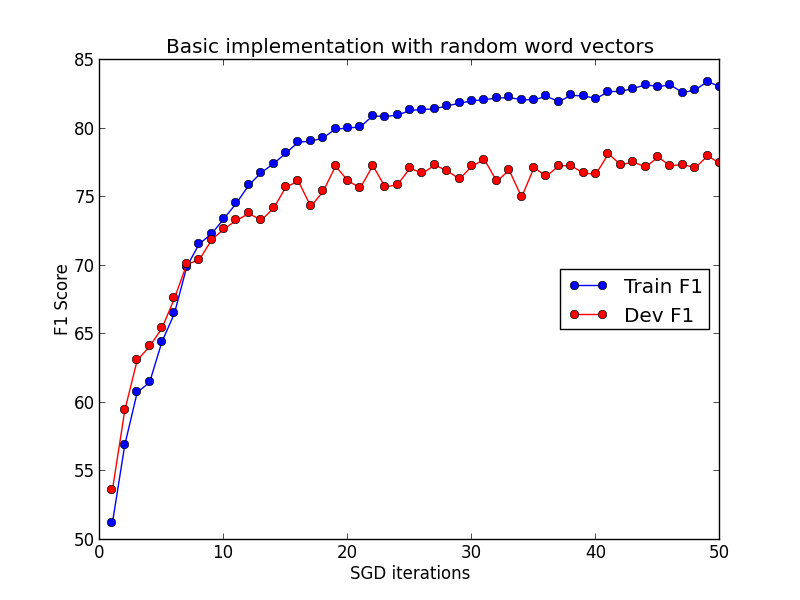
\includegraphics[width = \linewidth]{plots/baseline}
\caption{Learning curve for basic system}
\label{fig:basic}
\end{figure}
As shown in Figure~\ref{fig:basic}, we see that the training performance goes up steadily as expected, while the dev F1 stagnates at about 20 epochs. Overfitting becomes significant towards the end. Peak dev F1 score is 76.67, with corresponding training F1 82.64 and test F1 75.88.

At this point, we compare the pre-trained word vectors with random word vectors. For this, we generated 50-dimensional vectors randomly for all words, and plot the learning curve as follows:
\begin{figure}[H]
\centering
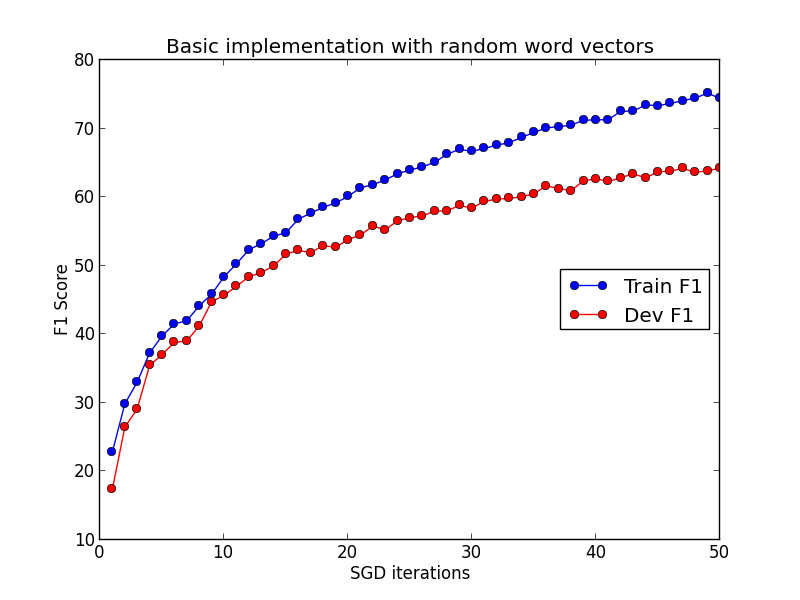
\includegraphics[width = \linewidth]{plots/randomwv}
\caption{Learning curve for random WV}
\label{fig:randomwv}
\end{figure}
Comparing the two graphs, we see that using random word vectors gives a much slower start, while using the pretrained vectors allows the performance to peak out relatively early. Also, the end performance of using pre-trained vectors is also quite a bit better.

From these results, we hypothesize that it is because even though the word vectors were trained without NER in mind, the unsupervised training still captured common traits between words that help the NER task. Therefore, in a supervised training scenario, the neural network can quickly exploit those traits and achieve good performance. (Of course, as we backpropagate into $L$, these vectors will also be tweaked towards the goal of NER). On the other hand, for random word vectors, all the training will be supervised and starts from scratch, so it takes many more iterations and even then, the results are not as good. This shows that even unsupervised pre-training can help supervised tasks.

After this, we moved on to implement sequence modeling, deeper neural networks (though we chose not to use it in the end), and incorporated word vectors from the `glove' set. These will be documented in detail in Section 6. With these extra improvements, we are ready for parameter tuning.
\subsubsection{Learning Rate $\alpha$}
For the learning rate, we started with $\alpha = 10^-3$, which worked very well. We experimented with other values, but the end performance was quite similar.

One idea that we had was to have a variable learning rate, with high $\alpha$ at first to speed up earlier training and lower $\alpha$ towards the end to not overshoot the optimal value. The effects of that was quite good, and in future runs we would see that the F1 score exceeds 70 in just one iteration.

Another thing to mention is that since we are doing SGD instead of batch or mini-batch GD, we would do well to shuffle the order of the training examples for every epoch. In practice, this sped up the convergence speed and even added a bit (~0.01 F1) to the peak performance.
\subsubsection{Regularization Parameter $\lambda$}
Regularization helps prevent overfitting by making sure that the weights do not become too big. The larger $\lambda$ is, the stronger the effect. It is expected that with large $\lambda$, the training accuracy cannot rise as high as with little or no regularization. The training F1 of the first 3 iterations with different values of $\lambda$ are shown in Table~\ref{tab:lambda}. The trend is quite obvious from these numbers, and carry on throughout the training process.
\begin{table}[H]
\centering
	\begin{tabular}{|c|c|c|c|}
		\hline
		$\lambda$ & Iter. 1 & Iter. 2 & Iter. 3 \\\hline
		$5\times10^-3$ & 72.04 & 75.43 & 77.39 \\\hline
		$5\times10^-2$ & 71.62 & 75.16 & 77.14 \\\hline
		$5\times10^-1$ & 70.82 & 74.71 & 76.34 \\\hline
	\end{tabular}
	\caption{Training F1 for different $\lambda$}
\label{tab:lambda}
\end{table}
In the end, we chose $\lambda = 0.0005$ because it gave the best dev performance. However, the difference between the other options were in fact quite small.
\subsubsection{Hidden Layer Nodes}
The number of hidden layer nodes determines how expressive your neural network can be. If the number is too low, the network may underfit the data, while a large amount of training data would be needed to do well if the number is high.

For this parameter, we tried out $H=10,20,40,60,100$. The results are shown in Figure~\ref{fig:hidden}.
\begin{figure}[H]
\centering
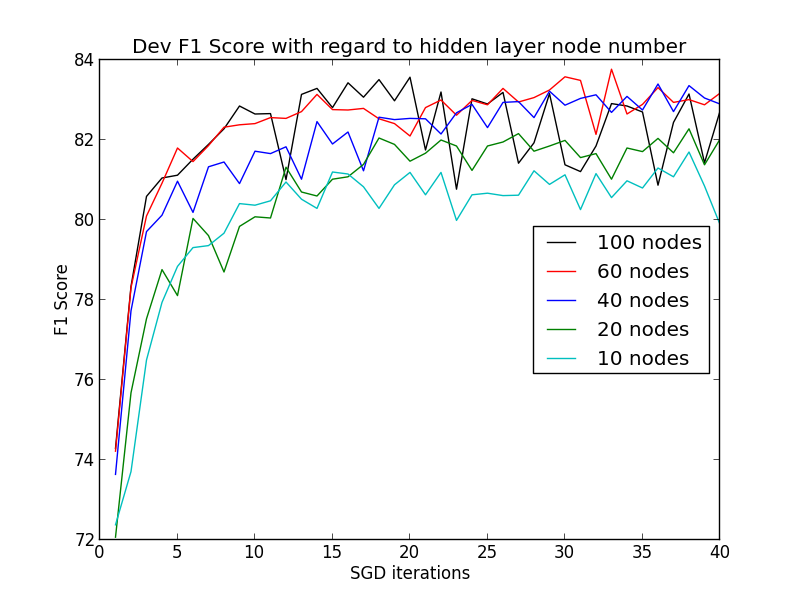
\includegraphics[width = \linewidth]{plots/hidden}
\caption{Dev F1 score for different H}
\label{fig:hidden}
\end{figure}
Figure~\ref{fig:hidden} is very interesting. For $H=20$ and $H=10$, we see that the dev F1 score is consistently worse then $H=40$. It seems that the low number of hidden layer nodes cannot fully capture the information available in the data, and, as expected, it is worse for $H=10$ than for $H=20$.

Going into the middle region, we see that $H=40$ and $H=60$ both perform well. The values do not oscillate much between iterations, and are consistently good. One phenomenon is that the larger the $H$, the faster the F1 score ramps up -- this may show that a larger number of hidden nodes makes it easier for the network to fit the data.

Finally, we look at $H=100$. From the figure it seems that the performance is oscillating between iterations. Since this is not seen on for smaller hidden layer sizes, it suggests that with the amount of data we currently have, $H=100$ is too large, so the network is overfitting the training data, so the results on the dev set are not consistent.
\subsubsection{Window Size $C$}
The window size should be closely discussed along with the hidden layer size. The larger the window, the larger the input vector dimensions, which intuitively warrants more hidden layer nodes.

In our experiment, we tried $C=1,3,5,7$.
\begin{table}[H]
\centering
	\begin{tabular}{|c|c|}
		\hline
		Window Size & Max Dev F1 \\\hline
		1 & 81.18 \\\hline
		3 & 83.77 \\\hline
		5 & 83.12 \\\hline
		7 & 82.11 \\\hline
	\end{tabular}
	\caption{Dev F1 for different window sizes}
\label{tab:window}
\end{table}
Intuitively, if the window size is 1, you're looking at no context, so useful information is lost, hence the lower score. On the other hand, if the window size is too large, your input is larger, but might not supply enough information to justify the additional dimensions. In real life, you probably don't need to look 3 words ahead and behind to determine an NER type. The extra dimensions only hurt by making the problem bigger.
\subsection{Result}
In the end, Our system had variable learning rate ($\alpha = 0.002\rightarrow0.0005$), $\lambda = 0.0005$, $H=60$, and $C=3$. Along with the `glove' word vectors and sequence modeling, this gave us the best performance on the dev set.

The learning curve of such a system is shown in Figure~\ref{fig:result}. We see that the dev F1 score peaks at epoch 33, so our final system would be trained for 33 iterations.

Training and dev scores are shown below:
\begin{table}[H]
\centering
	\begin{tabular}{|c|c|c|}
		\hline
		Dataset & Train & Dev \\\hline
		Accuracy(\%) & 97.07 & 96.11 \\\hline
		Precision(\%) & 88.67 & 87.22 \\\hline
		Recall(\%)  & 87.22 & 80.59 \\\hline
		F1 & 86.40 & 83.77 \\\hline
	\end{tabular}
	\caption{Final System Performance}
\label{tab:result}
\end{table}
\begin{figure}[H]
\centering
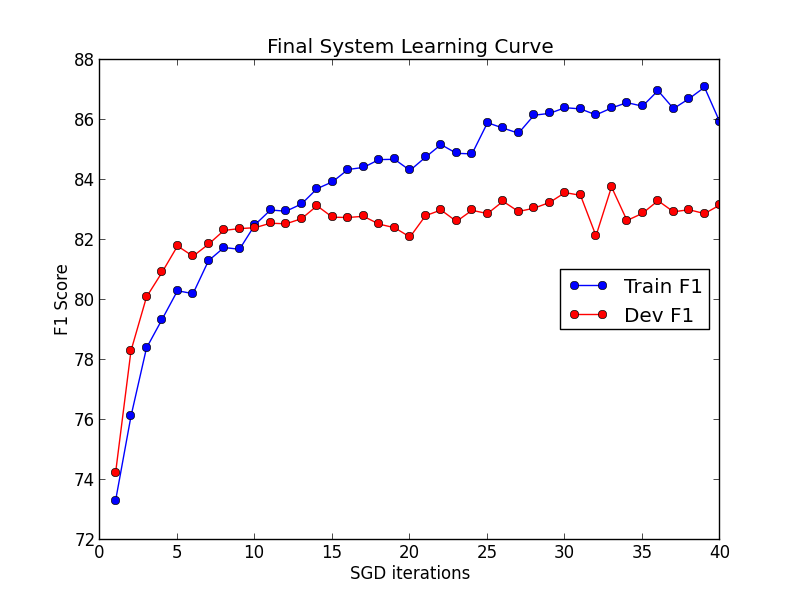
\includegraphics[width = \linewidth]{plots/result}
\caption{Learning Curve for Final System}
\label{fig:result}
\end{figure}
Finally, we trained our system and tested it on the hidden test set. The test accuracy was 95.12\% and F1 was 80.41. More detailed results are as follows:
\begin{table}[H]
\centering
	\begin{tabular}{|c|c|c|c|}
		\hline
		Tag & Prec. & Recall & F1 \\\hline
		\textbf{Total} & \textbf{81.44} & \textbf{79.41} & \textbf{80.41}\\\hline
		LOC & 78.69 & 81.51 & 80.07 \\\hline
		MISC & 73.41 & 67.97 & 70.59 \\\hline
		ORG  & 73.53 & 71.55 & 72.53 \\\hline
		PER & 93.40 & 88.82 & 91.05 \\\hline
	\end{tabular}
	\caption{Test Set Performance}
\label{tab:test}
\end{table}
\subsection{Error Analysis}
Firstly, we created a confusion matrix for the final results, which was very useful to gain an overview of the system's performance:
\begin{table}[H]
\centering
\begin{tabular}{|c|c|c|c|c|c|}
		\hline
		 & O & LOC & MISC & ORG & PER \\\hline
		O & 37945 & 85 & 148 & 288 & 88 \\\hline
		LOC & 80 & 1569 & 16 & 234 & 26 \\\hline
		MISC & 186 & 34 & 624 & 56 & 18 \\\hline
		ORG & 338 & 268 & 62 & 1786 & 42 \\\hline
		PER & 207 & 38 & 0 & 65 & 2463 \\\hline
	\end{tabular}
	\caption{Confusion Matrix}
\label{tab:confusion}
\end{table}
From the confusion matrix, we see that the system generally does very well (the biggest numbers are on the diagonals), but it is prone to make two kinds of mistakes:
\begin{enumerate}
\item
The system gets wrong whether a word is a named entity: We see that the first row and first column have many of the largest error counts.

Considering the fact that the vast majority of words in the data are not named entities, it is indeed a tough problem to tell whether the word should be in one of the four categories at all. We see that the false negatives and false positives have around the same number (609 vs 811), so the system is not leaning toward any particular side.
\item
The system has trouble differentiating between ORG and LOC.

234/1925 of `LOC' were classified as `ORG', while 338/2496 of `ORG' were classified as `LOC'. These two stand out as easily the two most common types of errors made by our system (excluding the `O's). They both occur almost ten times more frequently than other errors between named entity types.

Intuitively, it is indeed possible that these two types are hard to differentiate. For example, `the United States' should be classified as three `LOC's, but `the United States Navy' becomes four `ORG's.

In order to combat this, we could feed the system some better training examples that address this confusion. Also, we might need a bigger window size -- more information might be able to help differentiate in these conditions.
\end{enumerate}
Next, we look at some concrete examples:

(format: word, gold, predicted):
\begin{enumerate}
\item
\begin{verbatim}
United   I-LOC  I-ORG
Arab     I-LOC  I-LOC
Emirates I-LOC  I-ORG
\end{verbatim}
This is the case of confusing `LOC' with `ORG' that was mentioned previously. It is rather common. Looking at this specific example, perhaps a larger window size, as well as better sequence modeling would have helped.
\item
\begin{verbatim}
Igor     I-PER  I-PER
Shkvyrin I-PER  O
\end{verbatim}
For this example, it may be the case the `Shkvyrin' was not in the word vectors, so it was just an `UNK' vector. In that case, there was little the system could do. Again, better sequence modeling, or perhaps a huge word vector library (perhaps geared towards NER, so it includes more names) would have helped.
\item
\begin{verbatim}
Yasuto  I-PER  O
Honda   I-PER  I-ORG
\end{verbatim}
`Yasuto' was probably not in the word vectors, while `Honda' got classified as an `ORG'. A very understandable mistake, since `Honda' is also an organization. More context needed to make a correct classification here.
\end{enumerate}
\section{Extra Credit}
\subsection{Compare Word Vectors}
We downloaded the glove word vectors \textit{glob.6B.50d.txt} and converted it to the format similar to the given word vectors and vocabulary list files. We also added the special symbols $UUUNKKK$, $\langle s\rangle$, and $\langle /s\rangle$ to make it consistent with the given word vectors. As mentioned in Section 2, the new word vectors significantly improved our performance.

We believe that the glove word vectors was helpful in performance because of its significantly large word collections, which includes 4 times as many as words as the original word vectors. Therefore, more words will be trained with actual vectors instead of being discarded as unknown words.

\subsection{Sequence Modeling}
We added an interface to support sequence modeling. In sequence modeling mode, the dimension of the following matrices changed, where $K$ is the number of label classes.
\begin{table}[H]
\centering
	\begin{tabular}{|l|c|c|}
		\hline
		 & Old Dimensions & New Dimensions \\\hline
		$x$ & ${(nC+1)}\times{1}$ & ${(nC+1+K)}\times{1}$ \\\hline
		$W$ & ${H}\times{(nC+1)}$ & ${H}\times{(nC+1+K)}$ \\\hline
	\end{tabular}
\caption{Dimensions with Seq. Modeling}
\label{tab:dim2}
\end{table}
We initialized $W$ and $x$ accordingly. Starting from the first iteration, we stored the prediction vector $p$ and input the values to vector $x$ in the next iteration. Sequence modeling also gave slightly better performance, so we kept it in our final system.
\subsection{Deeper Networks}
For this part, we added an extra hidden layer to our neural network. The implementation was very similar to the original system, but there was an extra layer in the feedforward process as well as backpropagation.

Feedforward now uses the following:
\begin{equation*}
p_\theta(x)=g(Uf(W^{(2)}f(W^{(1)}x + b^{(1)})+b^{(2)})+b^{(3)})
\end{equation*}
Meanwhile, backpropagation gets gradients:
\begin{gather*}
\delta^{(3)} = p_\theta(x) - y\\
\delta^{(2)} = U^T\delta^{(3)}\circ(1-h^{(2)2})\\
\delta^{(1)} = W^{(2)T}\delta^{(2)}\circ(1-h^{(1)2})\\
\delta^{(0)} = W^{(1)T}\delta^{(1)}\\
\frac{\partial J(\theta)}{\partial U} = \delta^{(3)}h^{(2)T}, \frac{\partial J(\theta)}{\partial b^{(2)}} = \delta^{(3)}\\
\frac{\partial J(\theta)}{\partial W^{(2)}} = \delta^{(2)}h^{(1)T}, \frac{\partial J(\theta)}{\partial b^{(1)}} = \delta^{(2)}\\
\frac{\partial J(\theta)}{\partial W^{(1)}} = \delta^{(1)}x^T, \frac{\partial J(\theta)}{\partial b^{(1)}} = \delta^{(1)}\\
\frac{\partial J(\theta)}{\partial x} = \delta^{(0)}\\
\end{gather*}
These gradients also pass the gradient check mentioned in Section~1.6.

Using a deeper network means that there is one extra parameter, the size of the second hidden layer. We did some experiments and ended up choosing $H1=60,H2=20$.

With these parameters, our deeper network got a Dev F1 score of 83.41 after training for 26 iterations. The test F1 for such a system was 79.68, which was quite decent, especially considering that we did not do much parameter tuning.

However, the deeper system was slower to train and had more parameters to tune, so we focused on the shallow network in our report.
\section{Further Improvements}
In addition to what we have talked about in the analysis for Section 2, there are still things we can try to improve the scores.

One idea is that we could train 3-5 systems with different parameters and form an ensemble to `vote for' the final tag prediction. These methods have been known to push scores higher.

\end{document}